\chapter{Additive mixed models with kernel smoothers}

	\section{Introduction}
	\label{s:intro}
	% the problem of interest
	Geographically heterogeneous disease rates are of common interest in epidemiology studies since local high or low rates may serve as a surrogate for space-related risk factors such as environmental exposures and local healthcare access or quality. Traditional geographic modeling methods focus on analyzing aggregated area-level data that treat area-defined partitions as one unit. More recent spatial epidemiology studies avoid aggregation bias and the ecological fallacy by modeling individual-level data that may be collected longitudinally over time.  With accurate records of geospatial information (frequently longitude and latitude), researchers generally assume an underlying smooth surface for modeling the heterogeneity of disease risk over a given geospatial region, regardless of borders of inner areas. Based on this assumption, the estimation of the surface is an essential component in spatial data analysis. 
	
	Due to the complex nature of geospatial disease risk, it is not feasible to assume a parametric form to model the underlying risk surface in most cases. As such, nonparametric methods are popular in spatial effects modeling. Under a frequentist estimation framework, popular nonparametric methods include kernel and spline smoothers. Kernel smoothers utilize locally weighted models while spline smoothers are defined by a basis expansion of the design matrix over the full predictor support. In this work we consider locally weighted regression (LOESS) as proposed by \citet{cleveland1979robust}. LOESS assumes local (weighted) polynomial relationship between response and explanatory variables and was applied to geospatial analysis by \citet{brunsdon1996geographically} among others. One advantage of LOESS for spatial analyses is that it intuitively adapts to changing population densities by varying the size of the smoothing neighborhood based on the local data density given a fixed span size (typically defined as the proportion of observations used for local regressions). %One popular way to choose an optimal span size is to use Akaike information criterion (AIC). \citep{akaike1998information}
	
	In addition to spatial risk pattern estimation, confounding variables, such as biomarkers in studies on public health, should be included in spatial models. Generalized additive models (GAMs) \citep{hastie1990generalized} offer a framework for incorporating frequentist smoothers and confounding variables in an additive fashion by assuming a linear predictor consisting of the sum of nonparametric smoothers and parametric adjustment covariates. \citet{wood2017generalized} further developed GAMs by incorporating various types of splines and covered relevant topics such as computation, properties and applications. 
	
	Recently, data collection procedures such as patients revisits and health trackers have become increasingly prevalent. These procedures frequently result in multiple longitudinal measurements on individuals over time. This sampling framework results in within-subject correlation that must be accounted for in analytic methods in order to provide valid inferential results. Linear mixed models (LME) provide one framework for modeling within-subject correlation by adding random effects to linear models. Increased flexibility in the LME can be accomplished by incorporating random effects into a GAM framework. The resulting models are commonly known as generalized additive mixed models (GAMMs). \citet{lin1999inference} considered one strategy for the incorporation spline smoothers into the LME framework. To the best of our knowledge, however, no existing literature covers additive mixed models with kernel smoothers. The current manuscript seeks to fill this gap by propoposing a class of additive mixed models (AMM) that incorporate kernel smoothers and random effects into a linear model for continuous outcomes. 
	
	As one example, a fairly recent study was conducted to investigate serum perfluorooctanoic acid (PFOA) concentration among residents in Lubeck, West Virginia and Little Hocking, Ohio. \citep{bartell2010rate} In this study, researchers aimed to understand the declining behavior of PFOA concentration after granular activated carbon filtration on the public water systems in 2007. By design, 200 residents were included and 6 blood samples were to collect from each resident from May 2007 to August 2008 so that a trend of PFOA concentration could be observed. Besides PFOA concentration, residents' information such as gender, age and recent water consumption type (public water or bottled water) was recorded as well as precise residential location (recorded as longitude and latitude). One of the objectives is to understand the geospatial distribution of residents' serum PFOA concentration in order to help identify potential latent space-confounded risk factors. 
	
	The remainder of the manuscript is organized as follows: In Section 2, we introduce our proposed additive mixed models (AMMs) and the corresponding fitting procedure. In Section 3, we present simulation studies designed to assess the performance of our new model in geospatial risk pattern recreation and parameter estimation. In Section 4, we use our proposed methods on PFOA data to estimate the geospatial pattern in serum PFOA concentration in the area of Lubeck, WV. Finally, Section 5 provides further discussion about the proposed work and considers avenues of future research.
	
	\section{Methods}
	\label{s:Methods}
	\subsection{Notations}
	Let $i=1,2,\dots,N$ be the individual index where each $i$ corresponds to one individual. For each individual $i$, measurements are taken at times $t_{i1}, t_{i2},\dots,t_{iJ_i}$. The measurements on individual $i$ include the continuous response vector $Y_i=(y_{i1}, y_{i2}, \dots, y_{iJ_i})$ and a length-$p$ vector of adjustment covariates $X_{ij}$ at time $t_{ij}$, $j=1,\dots,J_i$. In addition, each individual's geographical information (i.e. longitude and latitude) is tracked, labeled by $(u_{ij},v_{ij})$ at time $t_{ij}$. Independence is assumed between individuals but not between the repeated measurements within each individual in statistical analysis.
	
	  Let $j=1,\dots,J$, denote a discrete time index and $i=1,\dots,N$, denote the individual index. Let $Y_i=(y_{i1}, y_{i2}, y_{i3}, \dots, y_{iJ})$ denote the vector of continuous responses for individual $i$.  We assume independence between individuals while allowing for correlation between measurements on the same individual. In addition, we note that $Y_i$ does not need to be complete with length $J$. In other words, individuals might not be measured at all time points. Let $(u_{i},v_{i})$ denote the geospatial location (longitude and latitude) of observation $i$ across all time, and let the function $lo()$ denote a LOESS smoother. Finally, let $X_{ij}$ denote a length-$p$ vector of potential time-dependent adjustment variables corresponding to observation $i$ at time $j$. 
	
	\subsection{LOESS with variance-covariance adjustment (LOESS-VCA)}
	%The classic LOESS smoother was built on the idea that by applying local simple models, such as linear models, to the whole domain of interest, one could achieve a flexible fitted surface on the domain. For spatial risk pattern estimation, bivariate LOESS smoothers are frequently applied since these smoothers are designed to find the relationship between risk and a bivariate vector (longitude and latitude in spatial analysis). 
	
	We begin with a simple bivariate LOESS smoother for i.i.d. data given by
	\begin{equation} \label{mod:lo}
	y_{ij}=lo(u_{ij},v_{ij})+\epsilon_{ij},~~~i=1,\dots,N,~~~j=1,...J_i,
	\end{equation}
	where $\epsilon \stackrel{i.i.d.}{\sim} N(0,\sigma^2)$. In (\ref{mod:lo}), the mean response at location $(u^*,v^*)$, i.e. $lo(u^*,v^*)$, is the estimand of scientific interest.  The local regression model involves $k$ of the observed data points that are nearest to $(u^*,v^*)$ where $k$ is pre-specified according to the span size and distance is generally defined as Euclidean distance for determining nearest neighbors. Utilizing the nearest neighbor data, locally weighted regression is used to estimate $lo(u^*,v^*)$, where weights are assigned according to the distance between the neighbor and the target location $(u^*,v^*)$. A traditional choice of weight function is the tricube weight function given by 
	\begin{equation} \label{eq:tricube}
	w(d) = \begin{cases} \Big( 1-\frac{d^3}{[max(d)]^3} \Big)^3, &\mbox{for } d < max(d)\\
	0, & \mbox{for } d > max(d) \end{cases}.
	\end{equation}
	\noindent In (\ref{eq:tricube}), $d$ denotes the distance and $max(d)$ is the maximum of the $k$ distances corresponding to the nearest neighbors. Let $L^*$ denote the local design matrix constructed by the local values of $(u,v)$, $W_1^*$ denote a diagonal matrix with tricube weights of the local observations, and $Y^*$ denote the response values of the local observations. Then the fitted value $\hat{lo}(u^*,v^*)$ can be calculated using weighted least squares:
	\begin{equation} \label{eq:wls}
	\hat{lo}(u^*,v^*)=(1\ u^*\ v^*)(L^{*T}W_1^*L)^{-1}L^{*T}W_1^*Y^*
	\end{equation}
	
	The above estimation procedure assumes $\epsilon \stackrel{i.i.d.}{\sim} N(0,\sigma^2)$. However, as we aim to estimate spatial patterns using longitudinal data, this assumption does not generally hold since measurements within each individual will tend to be correlated rather than independent. Thus, we extend the simple LOESS smoother to accommodate correlated data with a known, or assumed, correlation structure. 
	
	We again consider the mean model specified in (\ref{mod:lo}) but release the i.i.d. assumption. Rather, we assume $\mathbf{\epsilon} \sim N(0,\Sigma)$ where $\Sigma$ is known and $\mathbf{\epsilon}=(\epsilon_1,\epsilon_2,\dots,\epsilon_N)'$. With known, or assumed, variance-covariance model $\Sigma$, the weighted least squares estimator given in (\ref{eq:wls}) can be modified to account for within subject clustering via incorporation of inverse-variance weights. Specifically, let $\Sigma^*$ denote the local components of $\Sigma$ defined by the span size.  Then a variance-covariance adjusted LOESS (LOESS-VCA) fit is given by
	\begin{equation} \label{eq:wlsgls}
	\hat{lo}(u^*,v^*)=(1\ u^*\ v^*)(L^{*T}W_1^{*1/2}\Sigma^{*-1}W_1^{*1/2}L)^{-1}L^{*T}W_1^{*1/2}\Sigma^{*-1}W_1^{*1/2}Y^*.
	\end{equation}
	
	Since $\Sigma$ (and hence $\Sigma^*$) are generally not known in practice, a generalized estimating equations (GEE) approach \citep{liang1986longitudinal} that assumes a working covariance structure and iteratively replaces $\Sigma$ with a method of moments estimator could be used.  We, however, are interested quantifying potential random effects variance components.  In the next section we consider a two-stage backfitting strategy for incorporating both random effects and adjustment covariates into the bivariate LOESS model.
	
	\subsection{An additive mixed model with kernel smoothers}
	As discussed in Section \ref{s:intro}, additive models are popular tool among spatial epidemiologists seeking to estimate spatial disease risk patterns while simultaneously adjusting for potential confounding factors. Specifically, the model given in (\ref{mod:amloess}) that assumes i.i.d. errors $\epsilon_i$ is commonly extended in non-longitudinal sampling settings to estimate  spatial effects with covariate adjustment via a parametric component $X_{i}\beta$, yielding a model of the form
	\begin{equation} \label{mod:amloess}
	y_{i}=lo(u_{i},v_{i})+X_{i}\beta+\epsilon_{i}.
	\end{equation}
	
	However, when the dataset of interest includes multiple measurements on some individuals, the independence assumption does not inherently hold. Since Model \ref{mod:amloess} does not take the potential correlation among the measurements into account, inefficient or incorrect inference could be yielded if Model \ref{mod:amloess} is adopted. 
	
	To account for within-individual correlation arising from longitudinal sampling of individuals over time, \citet{laird1982random} proposed a class linear mixed effects models (LMEs) given by 
	\begin{equation} \label{mod:lmm}
	y_{ij}=X_{ij}\beta+Z_{ij}\gamma_i+\epsilon_{ij},
	\end{equation}
	where it is assumed that $\gamma_i \sim N(0,D)$ and $\mathbf{\epsilon_i}=(\epsilon_{i1},\epsilon_{i2},\dots,\epsilon_{iJ_i})' \sim N(0,R)$, with $\gamma_i$ and $\epsilon_i$ independent. Typically, the fixed effects $X_{ij}\beta$ component of the linear predictor is used to model the scientific association of interest and adjust for potential confounding covariates, the random effects $Z_{ij}\gamma_i$ component is used to model individual-specific effects and the $\epsilon_{ij}$'s are assumed to be i.i.d. conditional upon the random effects. 
	
	A natural extension of (\ref{mod:amloess}) to the setting of longitudinal data is given by an additive mixed model of the form
	\begin{equation} \label{mod:ammloess}
	y_{ij}=lo(u_i,v_i)+X_{ij}\beta+Z_{ij}\gamma_i+\epsilon_{ij}.
	\end{equation}
	
	
	\noindent While estimation procedures for generalized additive mixed models with spline smoothers have been proposed (cf. \cite{lin1999inference}), to the best of our knowledge, no previous work covered model fitting procedures for an additive mixed model with kernel smoothers. Here we consider a novel generalizing of the backfitting algorithm proposed by \citet{breiman1985estimating} to estimate the model specified in (\ref{mod:ammloess}).  
	
	We begin with the classic backfitting algorithm (presented in Algorithm \ref{alg:bf}). The basic idea of Algorithm \ref{alg:bf} is to fit partial residuals using one component in the mean model given the fitted values of the rest components in an iterative way, and repeating until convergence. Based on this algorithm, we propose Algorithm \ref{alg:bfmm} to fit (\ref{mod:ammloess}). Specifically, we propose modifying Algorithm \ref{alg:bf} by replacing the linear model with a LME utilizing a specified variance-covariance structure as determined by the specification of the random effects and the LOESS with the previously discussed LOESS-VCA estimator utilizing the induced working variance-covariance structre from the LME. As a result, estimation of both the non-parametric and semi-parametric components of the fixed effects linear predictor in (\ref{mod:ammloess}) incorporate the assumed variance-covariance structure of the longitudinal data. 
	\begin{algorithm}[H]
		\caption{Backfitting algorithm for Model \ref{mod:amloess} (Gaussian response)}
		\label{alg:bf}
		\begin{algorithmic}
			\State Initialize $\hat{lo}_{ij}=0$, $\hat{f}_{ij}=0$ for all $i$, $j$. 
			($\hat{lo}_{ij}$ will be the fitted values of the bivariate spatial LOESS smoother and $\hat{f}_{ij}$ will be the fitted values of the parametric component $X_{ij}\beta$.)
			\While{ at least one of the estimates $\hat{lo}_{ij}$ and $\hat{f}_{ij}$ change by 0.01\%, } 
			\State Fit linear model $(y_{ij}-\hat{lo}_{ij})\sim X_{ij}\beta$ and get fitted values $\hat{f}_{ij}$ for all $i,j$. 
			\State Centralize the fitted values using $\hat{f}_{ij}=\hat{f}_{ij}-\underset{i,j} {\text{mean}}(\hat{f}_{ij})$.
			\State Fit LOESS smoother $(y_{ij}-\hat{f}_{ij}) \sim lo(u_{ij},v_{ij})$ and get fitted values $\hat{lo}_{ij}$ for all $i,j$. 
			\State Centralize the fitted values using $\hat{lo}_{ij}=\hat{lo}_{ij}-\underset{i,j} {\text{mean}}(\hat{lo}_{ij})$.
			% 		\For {$k$ from 1 to $p$}
			% 		\EndFor
			\EndWhile
		\end{algorithmic}
	\end{algorithm}
	\begin{algorithm}[H]
		\caption{Backfitting algorithm for Model \ref{mod:ammloess} (Gaussian response)}
		\label{alg:bfmm}
		\begin{algorithmic}
			\State Initialize $\hat{lo}_{ij}=0$, $\hat{f}_{ij}=0$ for all $i$, $j$. 
			($\hat{lo}_{ij}$ will be the fitted values of the bivariate spatial LOESS smoother and $\hat{f}_{ij}$ will be the fitted values of the parametric component $X_{ij}\beta$.)
			\While{ at least one of the estimates $\hat{lo}_{ij}$ and $\hat{f}_{ij}$ change by 0.01\%, } 
			\State Fit linear mixed model $(y_{ij}-\hat{lo}_{ij})\sim X_{ij}\beta + Z_{ij}\gamma_i$ and get fitted values $\hat{f}_{ij}$ for all $i,j$. 
			\State Centralize the fitted values using $\hat{f}_{ij}=\hat{f}_{ij}-\underset{i,j} {\text{mean}}(\hat{f}_{ij})$.
			\State Calculate the estimated variance-covariance matrix $V$ from the mixed model. 
			\State Fit LOESS-VCA smoother $(y_{ij}-\hat{f}_{ij}) \sim lo(u_{ij},v_{ij})$ using $V$ as the true variance-covariance matrix and get fitted values $\hat{lo}_{ij}$ for all $i,j$. 
			\State Centralize the fitted values using $\hat{lo}_{ij}=\hat{lo}_{ij}-\underset{i,j} {\text{mean}}(\hat{lo}_{ij})$.
			\EndWhile
		\end{algorithmic}
	\end{algorithm}
	
	\subsection{Quantification of uncertainty in spatial effects}
	\label{s:Uncertain}
	Based on our proposed models, by using local weighted regression models, the estimated spatial effect at a specific location $(u^*,v^*)$ could be written as 
	\begin{equation} \label{eq:haty}
	\hat{lo}(u^*,v^*)=H^*(\Vec{\alpha})y^*,
	\end{equation}
	where $\vec{\alpha}=(D,R)^\prime$ stands for the variance component and $y^*$ would be the corresponding local response vector, which could potentially be the local working partial residual vector within the backfitting procedure if an AMM is being fitted. Hence the variance of $\hat{lo}(u^*,v^*)$ could be expressed as 
	\begin{equation} \label{eq:VarLO}
	Var(\hat{lo}(u^*,v^*))=H^*(\Vec{\alpha})Var(Y^*)H^{*T}(\vec{\alpha}),
	%=H^*(\hat{\alpha})V^*(\hat{\alpha})H^{*T}(\hat{\alpha})
	\end{equation}
	where $Var(Y^*)=V^*(\Vec{\alpha})$ is a function of $\Vec{\alpha}$ as well. We impute the estimated values of the variance component based on the linear mixed model and use
	\begin{equation} \label{eq:EVarLO}
	\widehat{Var}(\hat{lo}(u^*,v^*))=H^*(\hat{\Vec{\alpha}})V^*(\hat{\alpha})H^{*T}(\hat{\alpha})
	\end{equation}
	to quantify the uncertainty of the estimated spatial effects point-wisely. 
	
	\section{Monte Carlo studies}
	To assess the performance of our proposed methods in spatial effects estimation, we conducted multiple simulation studies based on a $2\times 2$ square map with a true  spatial pattern given by
	\begin{equation}\label{eq:nlsim}
	s_0(u,v) = -u + 0.1\log(1.3)v+1.2\sin(3(u+0.1))+2uv+ 6\log(0.6)v^2
	\end{equation}
	and depicted in the top plot of Figure \ref{f:simplots}. 
	
	\subsection{Spatial pattern recreation}
	In this section, we aimed to compare the performance of our proposed additive mixed models in terms of spatial pattern recreation. Responses were then simulated via the model
	\begin{equation}\label{eq:sim3}
	y_{ij} = s_0(u_{ij},v_{ij}) + b_{0i} + \epsilon_{ij},
	\end{equation}
	where $b_{0i} \stackrel{i.i.d.}{\sim} N(0,\sigma^2)$ and $\epsilon_{ij} \stackrel{i.i.d.}{\sim} N(0,1)$. We repeated the simulation with $\sigma^2=0,1.5,2.5$, respectively. %Under each scenario, we considered 1,000 simulated datasets for quantifying model performance
	
	% Figure 1 here
	
	We sought to compare our proposed additive mixed model (given in (\ref{mod:ammsim})) with a naive model that assumes independent data (given in (\ref{mod:amsim})):
	\begin{equation}\label{mod:ammsim}
	y_{ij} = \beta_0 + \beta_t t_{ij} + lo(u_{ij},v_{ij}) + b_{0i} + \epsilon_{ij}
	\end{equation}
	\begin{equation}\label{mod:amsim}
	y_{ij} = \beta_0 + \beta_t t_{ij} + lo(u_{ij},v_{ij}) + \epsilon_{ij}
	\end{equation}
	
	We compared the estimated spatial risk patterns between the 2 models under varying random intercept conditions. Span sizes that minimize AIC \citep{akaike1998information} were chosen for each model. Note that if $\sigma^2>0$, there will be individual-specific intercepts hence the model given in (\ref{mod:amsim}) is misspecified. It follows that the likelihood of Model (\ref{mod:amsim}) used in the AIC calculation would be incorrect hence the chosen span size might not be the most appropriate, however a search across different span sizes did not return qualitatively different results from what is presented here. 
	
	The estimated spatial risk patterns are shown in the second and third rows of Figure \ref{f:simplots}. It is easily seen that that with correctly specified random effects, our proposed additive mixed models estimate the spatial patterns in each scenario (bottom row). In contrast, since the naive additive model fails to account for within-subject correlation, results for the model given in (\ref{mod:amsim}) tend to under-smooth the patterns using a relatively small span size (second row). This is due to the fact that the naive additive model treats correlated data as independent, resulting in an improper contribution to the total likelihood. 
	
	\begin{figure}[H]
		\centering
		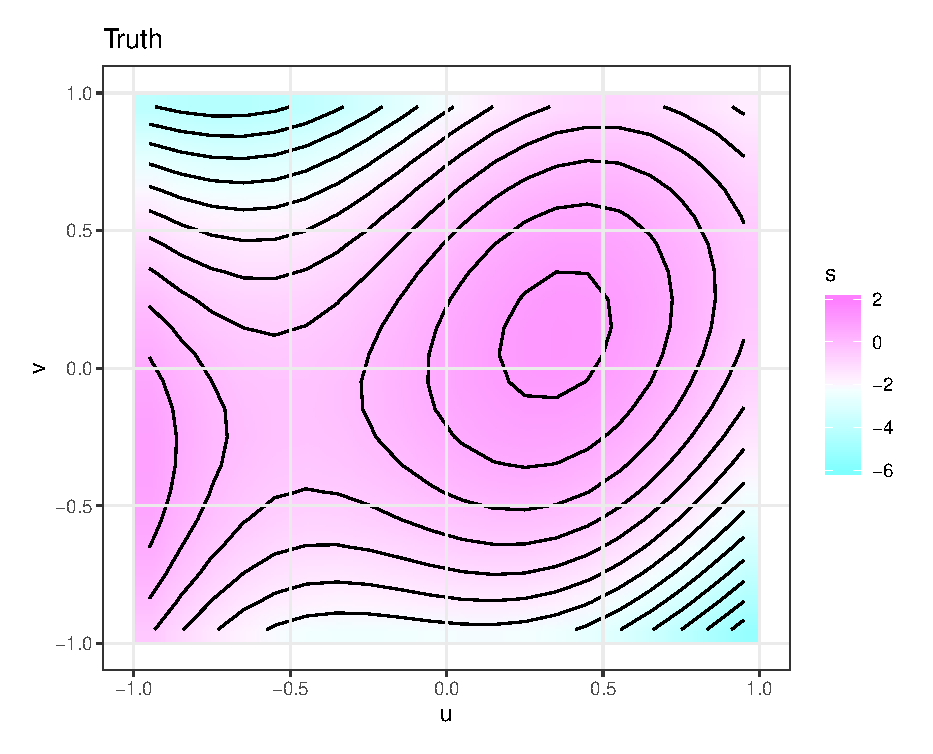
\includegraphics[width=0.33\linewidth]{Figures/Chap4/WNAR_true.eps}
		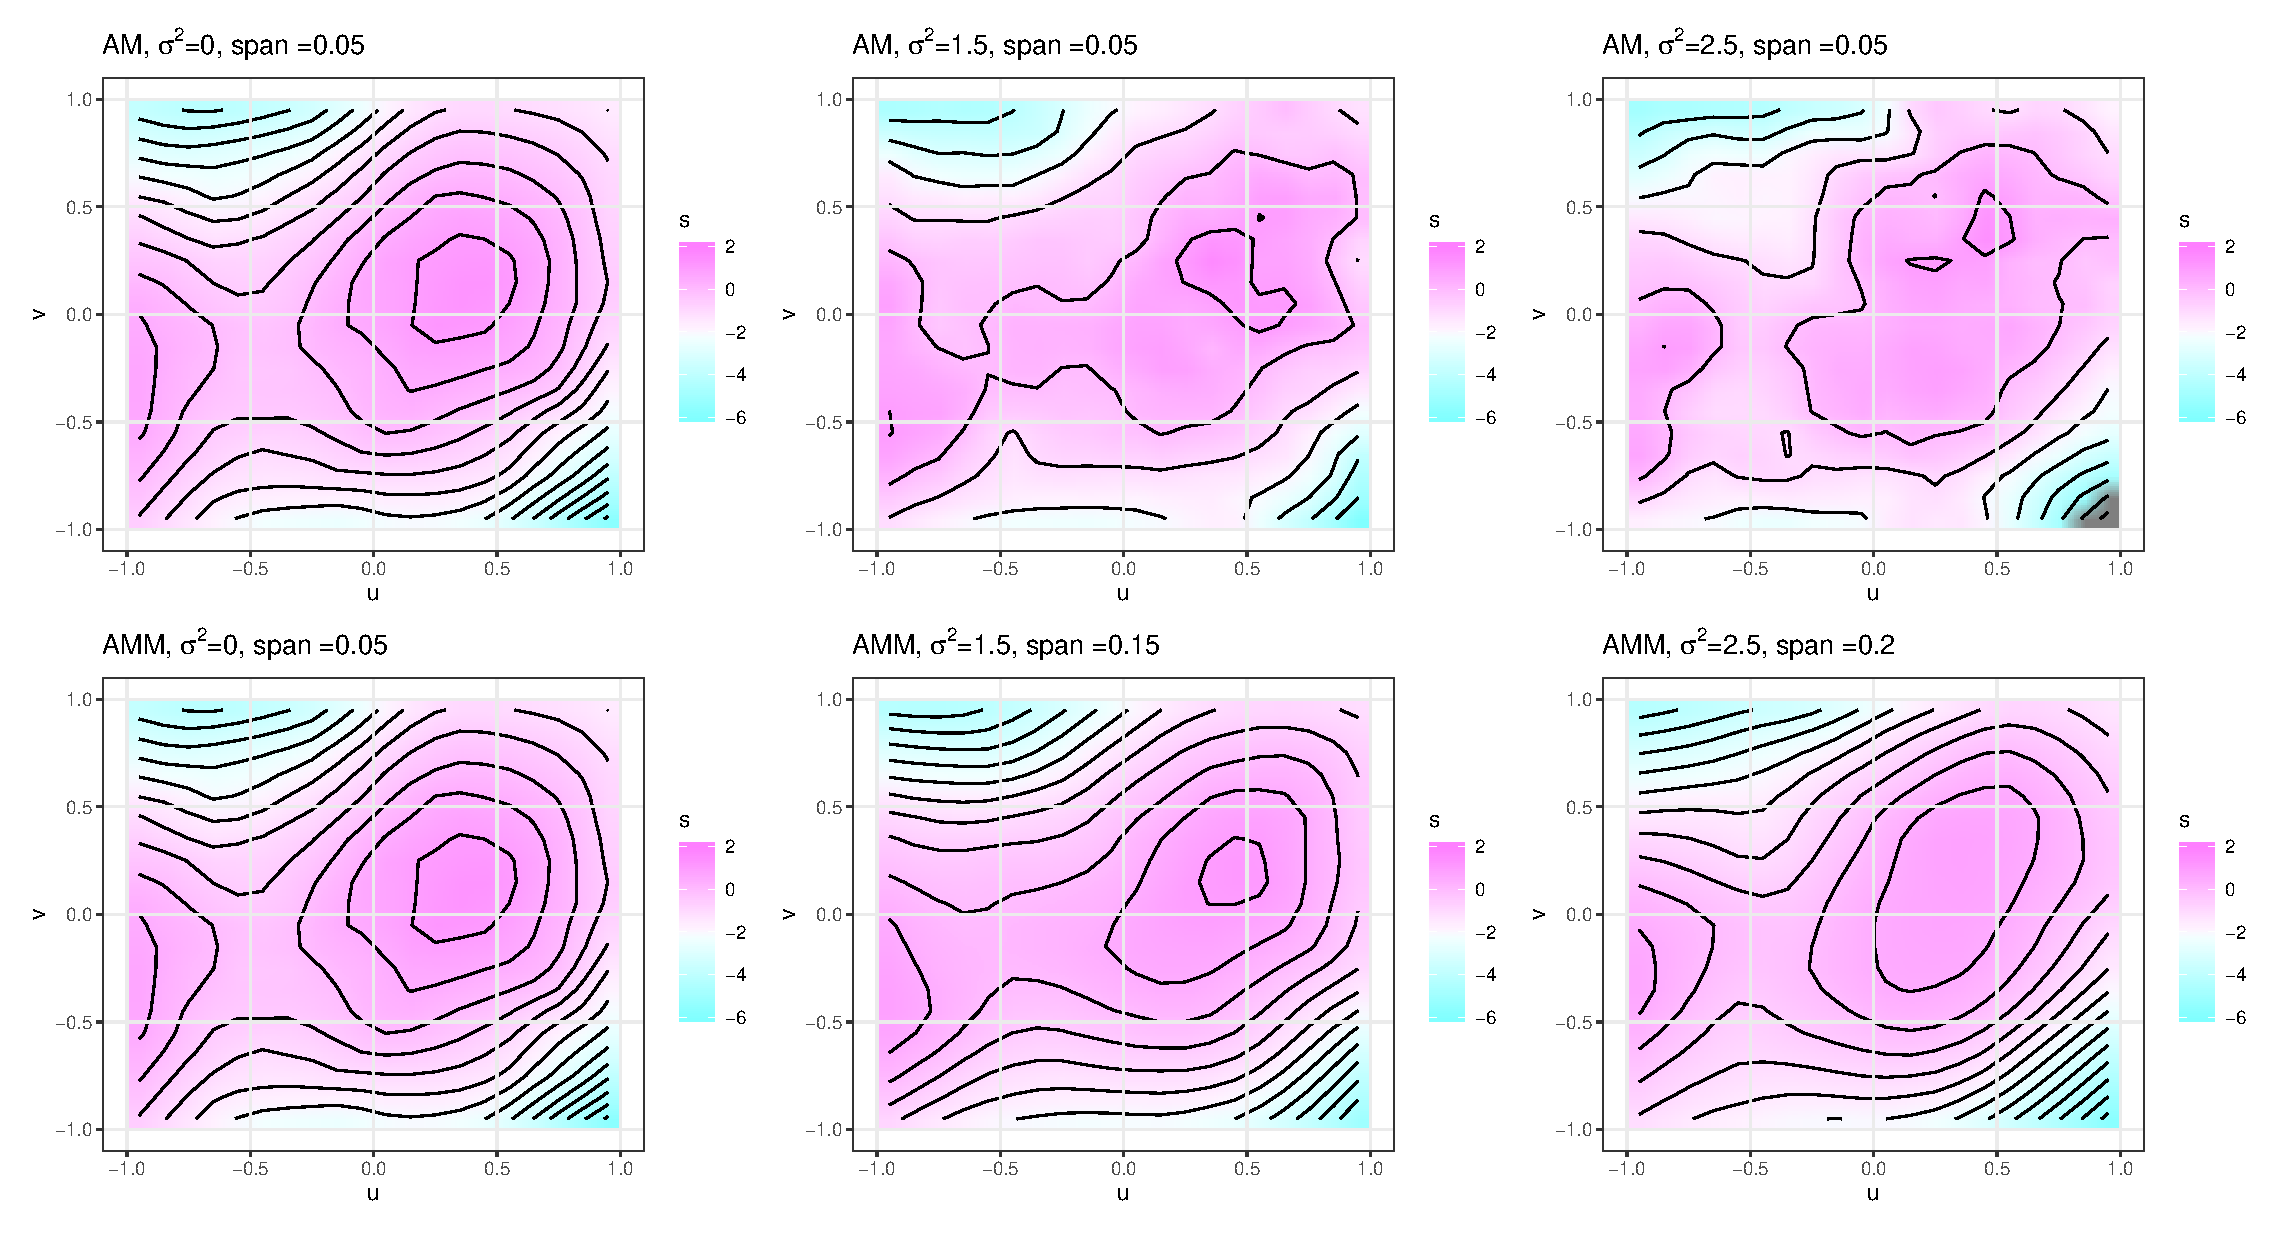
\includegraphics[width=\linewidth]{Figures/Chap4/WNAR_ests_h.eps}
		\caption{Top: Simulated spatial risk pattern; Middle: estimated patterns using additive models given differing correlation structures; Bottom : estimated patterns using additive mixed models given differing correlation structures.}
		\label{f:simplots}
	\end{figure}
	
	Similar simulations were conducted for scenarios where both random intercepts and random slopes exist. With random slopes included, we simulated data using 
	\begin{equation}\label{eq:simbothrand}
	y_{ij} = s_0(u_{ij},v_{ij}) + b_{0i} + b_{1i}t_{ij} + \epsilon_{ij},
	\end{equation}
	where $b_{0i} \stackrel{i.i.d.}{\sim} N(0,1.5)$, $b_{1i} \stackrel{i.i.d.}{\sim} N(0,\sigma_1^2)$ and $\epsilon_{ij} \stackrel{i.i.d.}{\sim} N(0,1)$. We repeated the simulation with $\sigma_1^2=0,0.04,0.09$, respectively. To these simulated data, we applied our proposed AMM (given in (\ref{mod:ammsim2RIRS})) and the same naive model that assumes independent data (given in (\ref{mod:amsim})).
	\begin{equation}\label{mod:ammsim2RIRS}
	y_{ij} = \beta_0 + \beta_t t_{ij} + lo(u_{ij},v_{ij}) + b_{0i} + b_{1i}t_{ij}  + \epsilon_{ij}
	\end{equation}
	
	From the recreated spatial risk patterns shown in Figure \ref{f:simplotsRIRS}, our proposed AMMs managed to deliver better performance with respect to selection of smoothing amount and pattern recreation when both random intercept and random slope exist and our model is accordingly specified.
	
	% Figure 2 here
	\begin{figure}[H]
		\begin{center}
			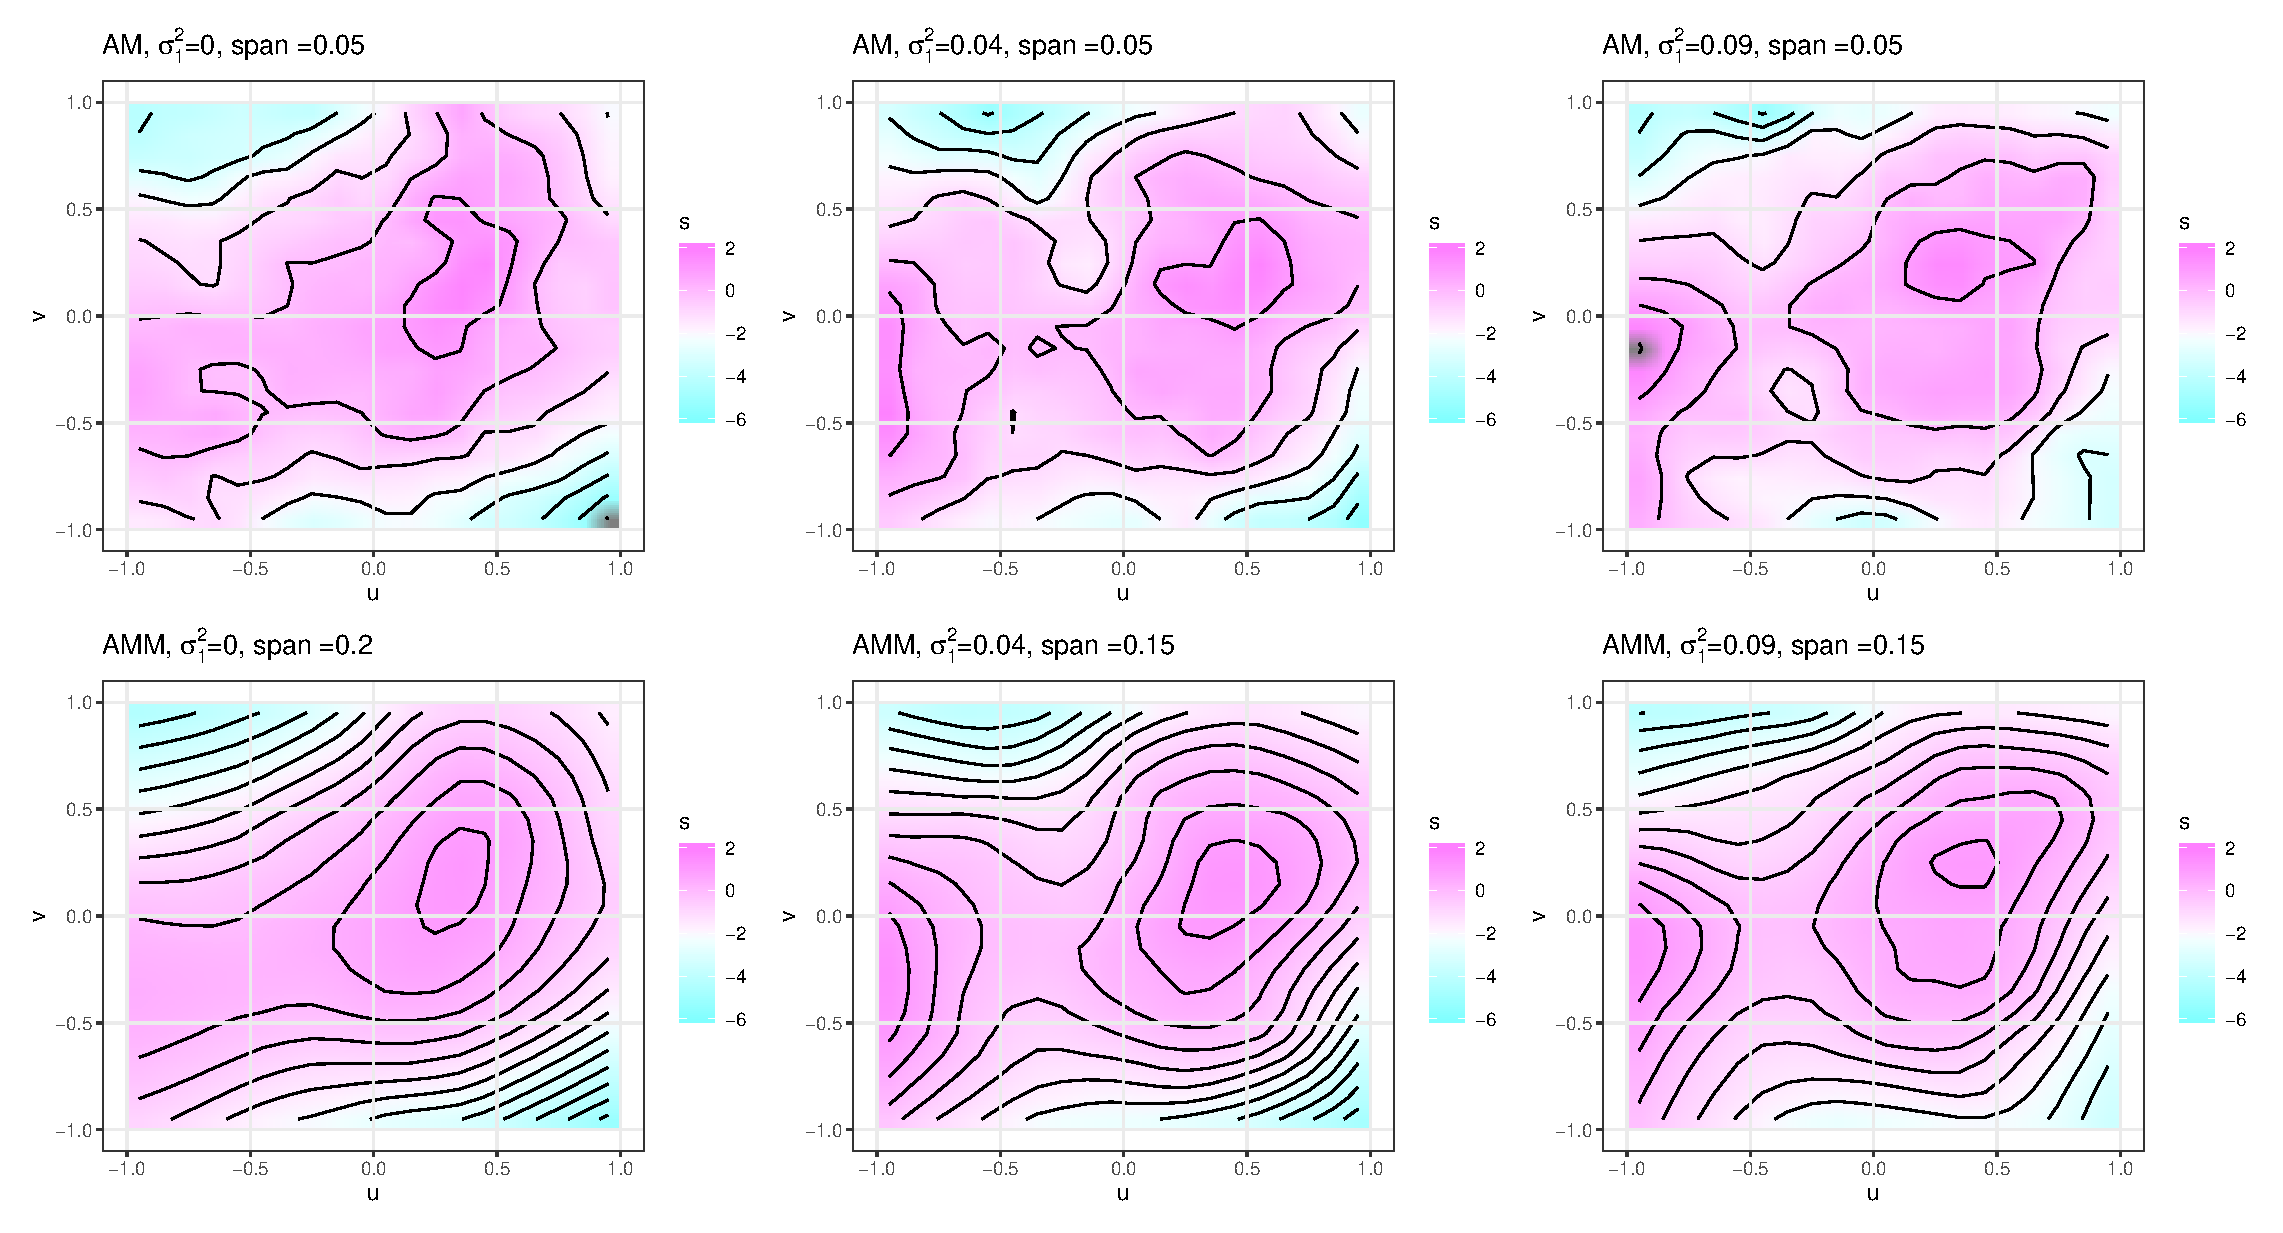
\includegraphics[width=\linewidth]{Figures/Chap4/WNAR_ests2_h.eps}
		\end{center}
		\caption{Top: estimated patterns using additive models given differing correlation structures; Bottom : estimated patterns using additive mixed models given differing correlation structures.}
		\label{f:simplotsRIRS}
	\end{figure}
	
	
	\subsection{Quantification of uncertainty of estimated spatial effects}
	To access the performance of our proposed methods to quantify the uncertainty of estimated spatial effects discussed in \ref{s:Uncertain}, simulated data were created using (\ref{eq:simbothrand}), where $b_{0i} \stackrel{i.i.d.}{\sim} N(0,1.5)$, $b_{1i} \stackrel{i.i.d.}{\sim} N(0,\sigma_1^2)$ and $\epsilon_{ij} \stackrel{i.i.d.}{\sim} N(0,1)$. Two scenarios were designed with $\sigma_1^2=0,\ 0.04$, respectively hence there were one scenario with random intercept only and one with both random intercept and random slope. 200 repetitions were performed for each scenario. For each repetition, 95\% CIs are derived using our proposed method for every location on a uniformly designed $20\times 20$ grid on the map. Both sample mean and sample standard deviation of the coverage were reported in Table (\ref{t:sim2coverage}). The empirical values of coverage are slightly less than 0.95, which might be due to the fact that although local weighted regressions manage to recreate a flexible spatial pattern in general, not every single piece of the true pattern could be precisely estimated with universal smoothing amount due to one single span size. However, the coverage probabilities were not far from 95\%, indicating that our proposed method does provide researchers with relatively meaningful inference on spatial effects. 
	
	% t:sim2coverage here
	\begin{table}[H]
		\caption{Sample mean and sample standard deviation of the coverage probability of confidence intervals of spatial effects based on 200 repetitions.
			\label{t:sim2coverage}}
		\centering
		\begin{tabular}{cccc}
			\hline
			$\sigma_0^2$ & $\sigma_{1}^2$ & mean coverage & s.d. \\
			\hline
			1.5 & 0 & 0.905 & 0.039\\
			1.5 & 0.04 & 0.879 & 0.065\\
			\hline
		\end{tabular}
	\end{table}
	
	
	\subsection{Parameter estimation}
	Here we investigate the performance of our proposed additive mixed model in terms of point estimation of the parameters in both the fixed effects and the variance of random effects via another set of simulation studies where responses were simulated using model 
	\begin{equation}\label{eq:simrand}
	y_{ij} = s_0(u_{ij},v_{ij}) + b_{0i} + b_{1i}t_{ij} + \epsilon_{ij},
	\end{equation}
	with $b_{0i} \stackrel{i.i.d.}{\sim} N(0,\sigma_{0}^2)$, $b_{1i} \stackrel{i.i.d.}{\sim} N(0,\sigma_{1}^2)$ and $\epsilon_{ij} \stackrel{i.i.d.}{\sim} N(0,\sigma_\epsilon^2)$. %Notably, we now assess the performance of the model when both a random intercept and random slope are present.
	
	On the simulated dataset, we sought to access the performance of our proposed AMM given by 
	\begin{equation}\label{mod:ammsim2}
	y_{ij} = \beta_0 + \beta_t t_{ij} + lo(u_{ij},v_{ij}) + b_{0i} + b_{1i}t_{ij} + \epsilon_{ij}.
	\end{equation}
	The estimated values of $\beta_t$, $\sigma_{0}^2$, $\sigma_{1}^2$ and $\sigma_\epsilon^2$ were recorded. Results presented in Table \ref{t:sim2paras} were based upon a total of 50 simulations. The sample mean and standard deviation of estimated model parameters were reported. From the results, it could be seen that our proposed AMMs managed to estimate parameters in both the mean and variance components in a consistent fashion.
	
	% t:sim2paras here
	% latex table generated in R 3.6.0 by xtable 1.8-4 package
	% Wed Jun 03 15:54:55 2020
	\begin{table}[H]
		\caption{Average and standard deviation of parameter estimates across 50 simulated datasets.\label{t:sim2paras}}
		\centering
		\begin{tabular}{llll}
			\hline
			parameter & truth & mean of estimates & s.d. \\ 
			\hline
			$\beta_t$ & 0.000 & -0.002 & 0.010 \\ 
			$\sigma_0^2$ & 1.500 & 1.428 & 0.133 \\ 
			$\sigma_1^2$ & 0.040 & 0.040 & 0.005 \\ 
			$\sigma_\epsilon^2$ & 1.000 & 0.989 & 0.028 \\ 
			\hline
		\end{tabular}
	\end{table}
	
	\section{Application to serum PFOA study}
	In this section, we apply our proposed additive mixed model to estimate the spatial pattern of residents' serum PFOA concentration with adjustment of relevant confounding covariates. Here we focus on a approximate square map defined within longitude  $81^{\circ} 30'\  W$ - $81^{\circ} 50'\  W$ and latitude $39^{\circ} 07'\  N$ - $39^{\circ} 27'\  N$, which is approximately a $23\times 23$ square in miles around Lubeck, WV area. Within this area, 1070 records on 193 individuals are available where 140 of them have 6 measurements of serum PFOA concentration. Among the 193 residents, 99 are female and 94 are male. Age at baseline has mean 54.6 and standard deviation 14.9 with minimum 19 and maximum 92.
	
	To estimate the spatial pattern of residents' serum PFOA concentration with control of gender, age and a linear trend in time, we fitted an AMM given by 
	
	\begin{equation}\label{mod:PFOA}
	log(PFOA)_{ij} = \beta_0 + \beta_1 female_i + \beta_2 age_i + \beta_3 t_{ij} + lo(u_{ij}, v_{ij}) +  b_{0i} + \epsilon_{ij}, 
	\end{equation}
	where $b_{0i} \stackrel{i.i.d.}{\sim} N(0,\sigma_0^2)$ and $\epsilon_{ij} \stackrel{i.i.d.}{\sim} \sigma_\epsilon^2$. 
	
	The fitted spatial pattern, along with point-wise 95\% confidence intervals, is shown in Figure \ref{f:pfoaplots}. From the results, it could be seen that potential high PFOA risk areas exist in western and northern part of the area. Further point-wise significance tests are performed at each location within a uniformly designed $20\times 20$ grid on the map of interest. Specifically, 95\% confidence interval of spatial effect at each location is compared with the mean estimated spatial effect over the 400 locations. A location is labeled as significant if the 95\% CI at the location does not cover the mean estimated effect. The results are plotted in Figure \ref{f:pfoasigs}, from which significantly higher risks are observed at 69 locations while significantly lower risks are observed at 103 locations, indicating significant geospatial disparity in residents' serum PFOA concentration over the map. These results could potentially help epidemiologists on further space-confounded risk factor detection. 
	
	% Fig f:pfoaplots here
	\begin{figure}[H]
		\begin{center}
			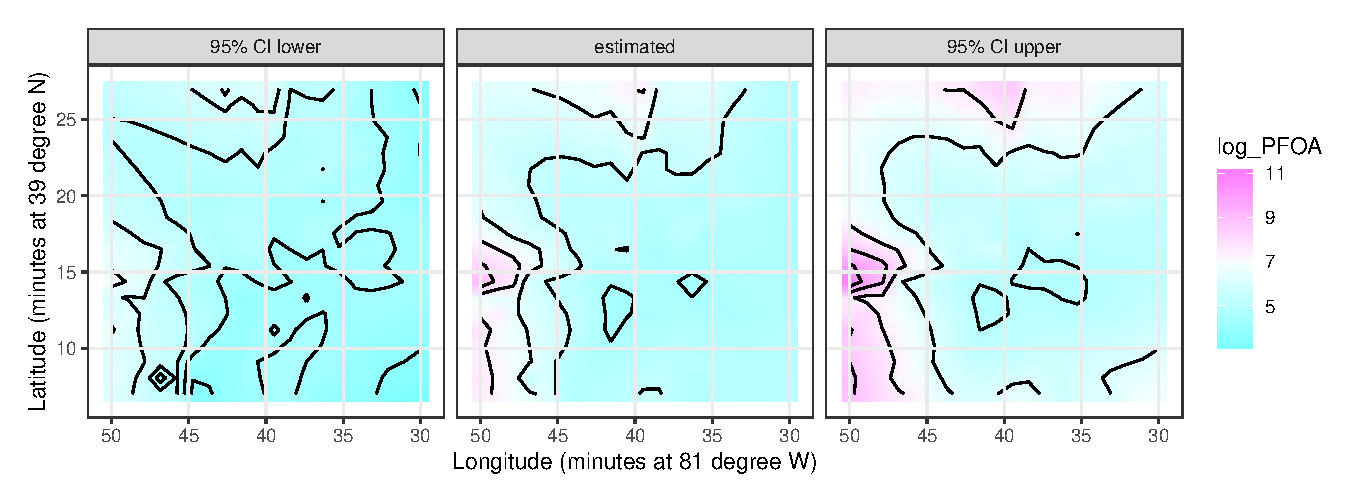
\includegraphics[width=\linewidth]{Figures/Chap4/PFOA_ests_55.eps}
		\end{center}
		\caption{Left: pointwise lower bounds of 95\% CIs ; Middle: estimated patterns using Model \ref{mod:PFOA}; Right: upper bounds of 95\% CIs.}
		\label{f:pfoaplots}
	\end{figure}

	% Fig f:pfoasigs here
	\begin{figure}[H]
		\begin{center}
			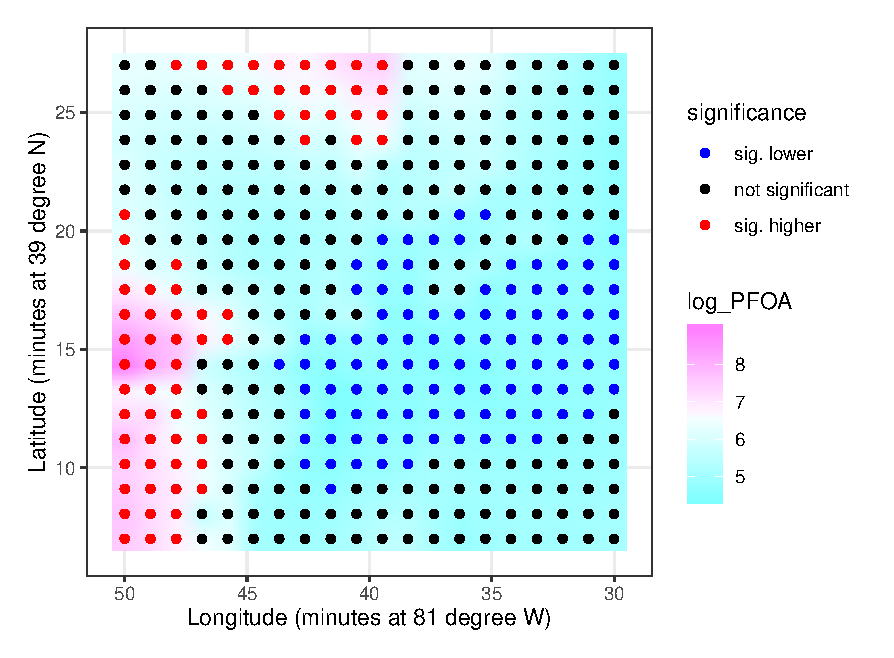
\includegraphics[width=0.5\linewidth]{Figures/Chap4/PFOA_sig.eps}
		\end{center}
		\caption{Significance of the grid locations on the estimated spatial effects map.}
		\label{f:pfoasigs}
	\end{figure}
	
	\section{Discussion}
	\label{s:discuss}
	We proposed a novel class of additive mixed models that incorporate kernel smoothers into the classic LME model. To achieve this, we first extended the LOESS smoother to adjust for a given variance-covariance structure and then proposed a new backfitting algorithm to fit the proposed additive mixed models using the extended LOESS (LOESS-VCA). Using Monte Carlo studies, we showed that our proposed additive mixed models managed to choose the proper amount of smoothing via AIC and estimate the underlying spatial risk patterns precisely, compared to corresponding naive additive models that assume independence. Empirical results also showed that our model consistently estimates parameters in both mean and variance components when the model is correctly specified. Our methods were further used in a recent study on residents' serum PFOA concentration in Lubeck, WV and spatial disparity in serum PFOA concentration was identified. 
	
	In this work, we focused on additive models with kernel smoothers, utilizing LOESS in particular. The motivation for this is to meet the demand of various spatial epidemiology studies. We mentioned but did not elaborate on the use of spline smoothers in the context of mixed models, partially because those models are relatively well investigated in existing literature. We did not consider Bayesian spatial estimation methods based on Gaussian processes but do recognize their popularity, as well.
	
	We consider this work as a first step to a complete set of generalized additive mixed models that incorporate kernel smoothing. We continue to work on relevant extensions. Specifically, we are currently extending the presented approach to the setting of additive mixed models for exponential family outcomes, such as binary and count responses. In this context a natural approach involves incorporation of kernel smoothing and PQL (penalized quasi-likelihood) \citep{breslow1993approximate} into the estimation procedure presented here.
	
%%% Local Variables: ***
%%% mode: latex ***
%%% TeX-master: "thesis.tex" ***
%%% End: ***
